\chapter{Miscellanea}

Le funzionalit\'a di cui sono pi\'u orgoglioso sono:
\\
1. Il server pu\'o far giocare potenzialmente infiniti giocatori.
\\
2. La matrice di gioco pu\'o essere N x N di dimensione arbitraria.
\\
3. Le parole possono avere lunghezza arbitraria.
\\
4. L'input dell'utente nel client pu\'o essere di lunghezza arbitraria.
\\
5. Le stampe nel client sono perfette, la GUI non mostra mai stampe incoerenti.
\\
6. I tests eseguiti mostrano una buona resa di server e clients.
\\
7. Il client e\' semplicissimo poich\'e il grosso del lavoro lo esegue \'e il server.
\\

La sincronizzazione \'e stata volutamente fatta solamente tramite mutex, dove talvolta le variabili di condizione o i semafori si sarebbero potuti utilizzare, per cercare di rendere il codice pi\'u semplice ed intuitivo possibile, seppur abbia ancora della complessit\'a.
\\
Quanti giocatori riesce a gestire nella pratica? Ci sono criticit\'a? Dai tests effettuati purtroppo si, nonostante come detto al punto 1, in teoria i giocatori potrebbero essere infiniti, vi \'e un problema. Quando si arriva all'incirca a 500 giocatori (attivi che fanno richieste), ma gi\'a dai 400, sulla macchina di laboratorio, un po' di pi\'u sul mio pc, il server diventa lentissimo nel rispondere ed accettare nuovi utenti paralizzando praticamente il gioco, questo a causa del fatto che sincronizzare 500 threads, considerando anche che in alcuni punti viene fatta attesa attiva (di cui mi sono pentito). Credo che il problema potrebbe essere parzialmente risolto aumentando di parecchio la priorit\'a (rispetto ai clientHandler() thread) dei thread signalsThread(), che gestisce i segnali ed il gioco, e quella del thread main che accetta i nuovi clients, ci ho provato molto, ma alla fine mi sono arreso perch\'e non riesco a farlo con le funzioni di scheduling dei pthreads.
 \\
 \\
 Le parole, indipendentemente da come arrivino dal client e da come siano scritte nei file dizionario vengono convertite in UPPERCASE dal server. Anche i caratteri componenti la matrice di gioco sono gestiti esclusivamente in UPPERCASE, sia nella generazione casuale, sia nella lettura da file (se scritte in lowercase in quest'ultimo vengono convertite in UPPERCASE). Gli unici caratteri ammessi per le parole, le matrici e i nickname degli utenti sono: \#define ALPHABET "abdcdefghijklmnopqrstuvxyz".
 \\
 L'input del client, invece, viene tutto convertito a lowercase prima di essere elaborato ed inviato, quindi il comando inserito "MaTrIcE" sarà valido come "matrice".
 
\begin{figure}[H]
    \centering
    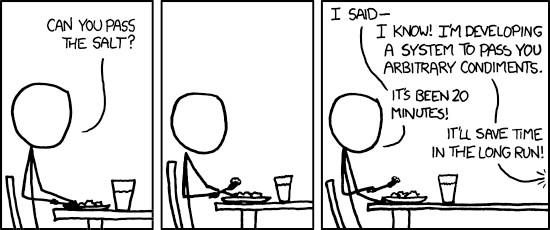
\includegraphics[scale=0.7]{meme.png}
    \caption{by XKCD}
\end{figure}